\documentclass[aspectratio=1610, professionalfonts, 13pt]{beamer}

% Lade das TU Dortund Theme von Max Nöthe
\usefonttheme[onlymath]{serif}
\usetheme[showtotalframes]{tudo}

% Lade richtiges Sprachpaket
\ifluatex
    \usepackage{polyglossia}
    \setmainlanguage{english}
\else
    \ifxetex
        \usepackage{polyglossia}
        \setmainlanguage{german}
    \else
        \usepackage[german]{babel}
    \fi
\fi

% Lade wichtige Mathematikpakete
\usepackage{amsmath}
\usepackage{amssymb}
\usepackage{mathtools}
\usepackage{cancel}
\usepackage[
  locale=DE,                   % deutsche Einstellungen
  separate-uncertainty=true,   % Immer Fehler mit \pm
  per-mode=symbol-or-fraction, % m/s im Text, sonst Brüche
]{siunitx}
\usepackage[absolute,overlay]{textpos}
\usepackage{framed}
\usepackage{multicol}
\usepackage{setspace}
\usepackage{graphicx}
\usepackage{booktabs}
\usepackage{caption}
\usepackage{appendixnumberbeamer}
\usepackage{tikz}
\usepackage[export]{adjustbox}
\usepackage{color}
\usepackage{animate}


% Lade Paket zur Nutzung von Schleifen
\usepackage{forloop}

% ------------------------- Präsentationsinformationen -------------------------

% Titel:
\title{\textbf{Analysis Of The Crab Nebula Using FACT's Photon Stream Data}}
% Autoren:
\author[K.\ Sedlaczek]{\textit{Kevin Sedlaczek}, Maximilian Nöthe for the FACT-Collaboration}


% Datum:
\date{20. March 2018}
\date[20. March 2018]{DPG-Frühjahrstagung 2018 Würzburg}
% Lehrstuhl/Fakultät:
\institute[TU Dortmund]{Lehrstuhl für Experimentelle Physik 5}

\institute[%
  {
\includegraphics[height=\headerheight]{logos/fact.pdf}}%
  \hspace{1em}%
  {
\includegraphics[height=\headerheight]{logos/e5logo.pdf}}%
]{
  {
\includegraphics[height=0.75cm]{logos/tu.pdf}}%
  \hspace{1em}%
  {
\includegraphics[height=0.75cm]{logos/ethz.pdf}}%
  \hspace{1em}%
  {
\includegraphics[height=0.75cm]{logos/isdc.pdf}}%
  \hspace{1em}%
  {
\includegraphics[height=0.75cm]{logos/uniwue.pdf}}%
}

% Titelgrafik:
% \titlegraphic{
\includegraphics[width=0.4\textwidth]{logos/FACTLogo_preliminary.png}\hfill
\includegraphics[width=0.4\textwidth]{logos/e5logo_green_text.pdf}}


\begin{document}

\maketitle

\section{The First G-APD Cherenkov Telescope}

\begin{frame}[t]{The First G-APD Cherenkov Telescope}
  % \begin{multicols}{2}
    % \vspace*{\fill}
    \begin{figure}
        \centering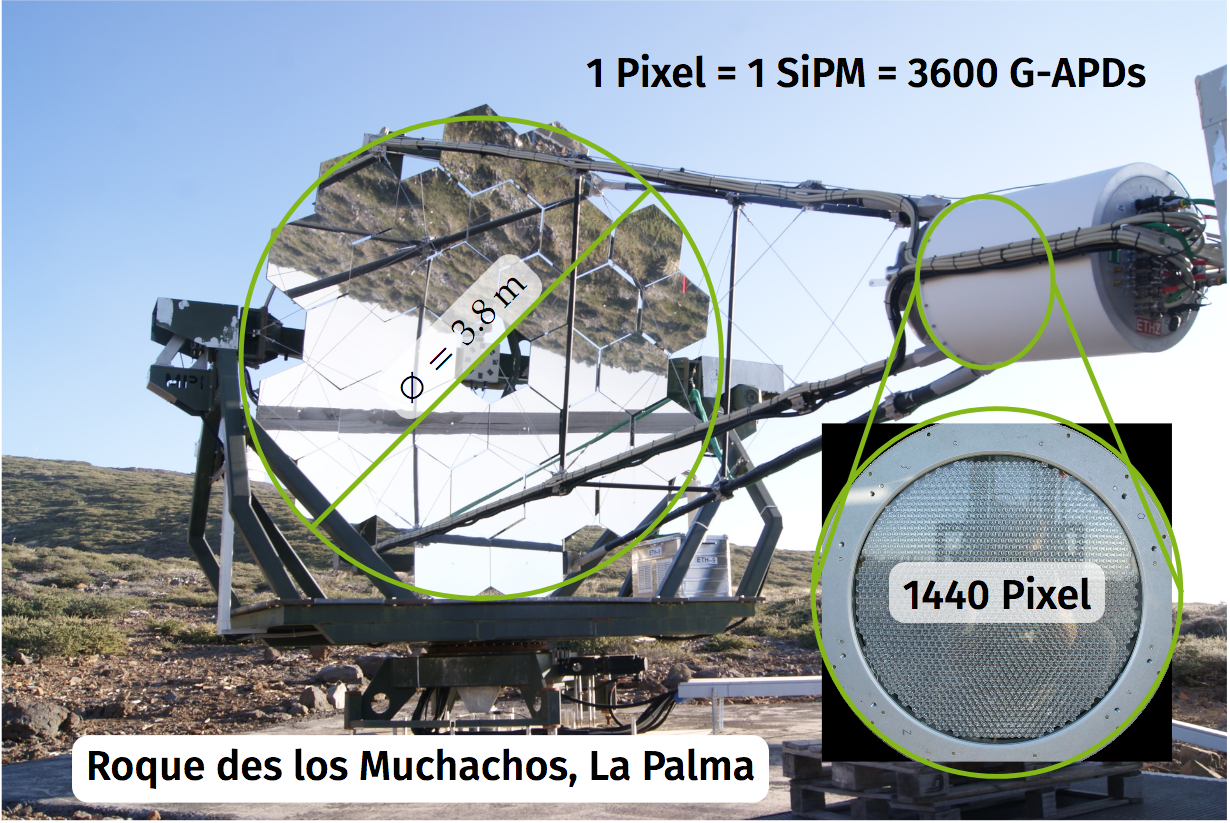
\includegraphics[width=0.65\textwidth]{fig/fact.png}
    \end{figure}
    % \columnbreak
    % \vspace*{\fill}
    %   \begin{itemize}
    %     \item located on Roque des los Muchachos, La Palma
    %     \item build to demonstrate novel light sensors \textit{silicon photo multipliers} (SiPM)
    %     \item offer possibility to operate under much brighter light conditions
    %     \item camera has single photon resolution
    % \end{itemize}
    % \vspace*{\fill}
  % \end{multicols}
\end{frame}

\section{Photon Stream}

\begin{frame}[t]{The Photon Stream Data}
\begin{columns}[onlytextwidth]
    \begin{column}{0.475\textwidth}
        \begin{overprint}
              \onslide<1>\vspace*{\fill}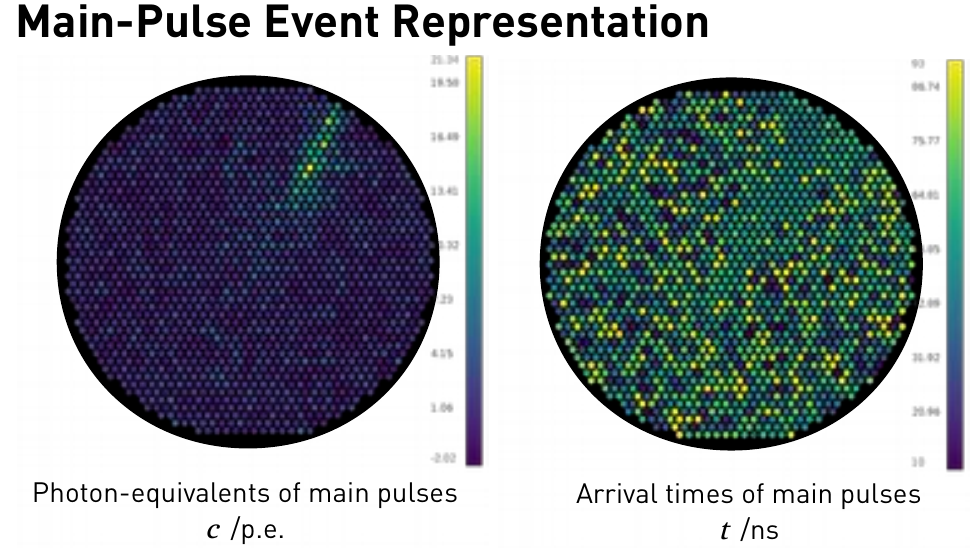
\includegraphics[width=\textwidth]{fig/standard.png}
              \onslide<2>\vspace*{\fill}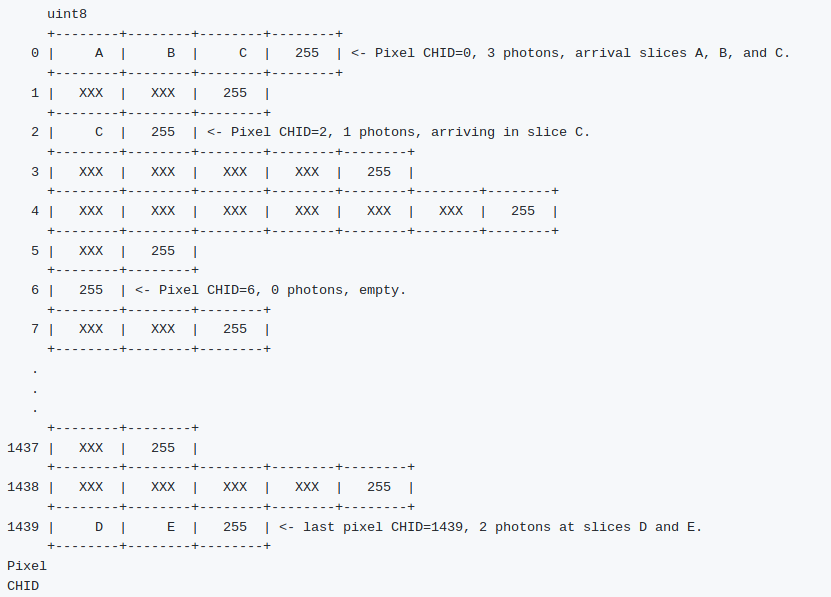
\includegraphics[width=\textwidth]{fig/lol.png}
        \end{overprint}
  \end{column}
  \begin{column}{0.475\textwidth}
      \begin{itemize}
          \item FACT records data in format close to readout hardware
          \item superposition of multiple photon signals
          \item not intended as physics format \\ $\rightarrow$ \textbf{Photon Stream}
          \item list of individual photons (arrival times)
      \end{itemize}
  \end{column}
\end{columns}

\end{frame}

\begin{frame}[t]{The Photon Stream Data}
\begin{columns}[onlytextwidth]
    \begin{column}{0.475\textwidth}
        \begin{overprint}
            \onslide<1>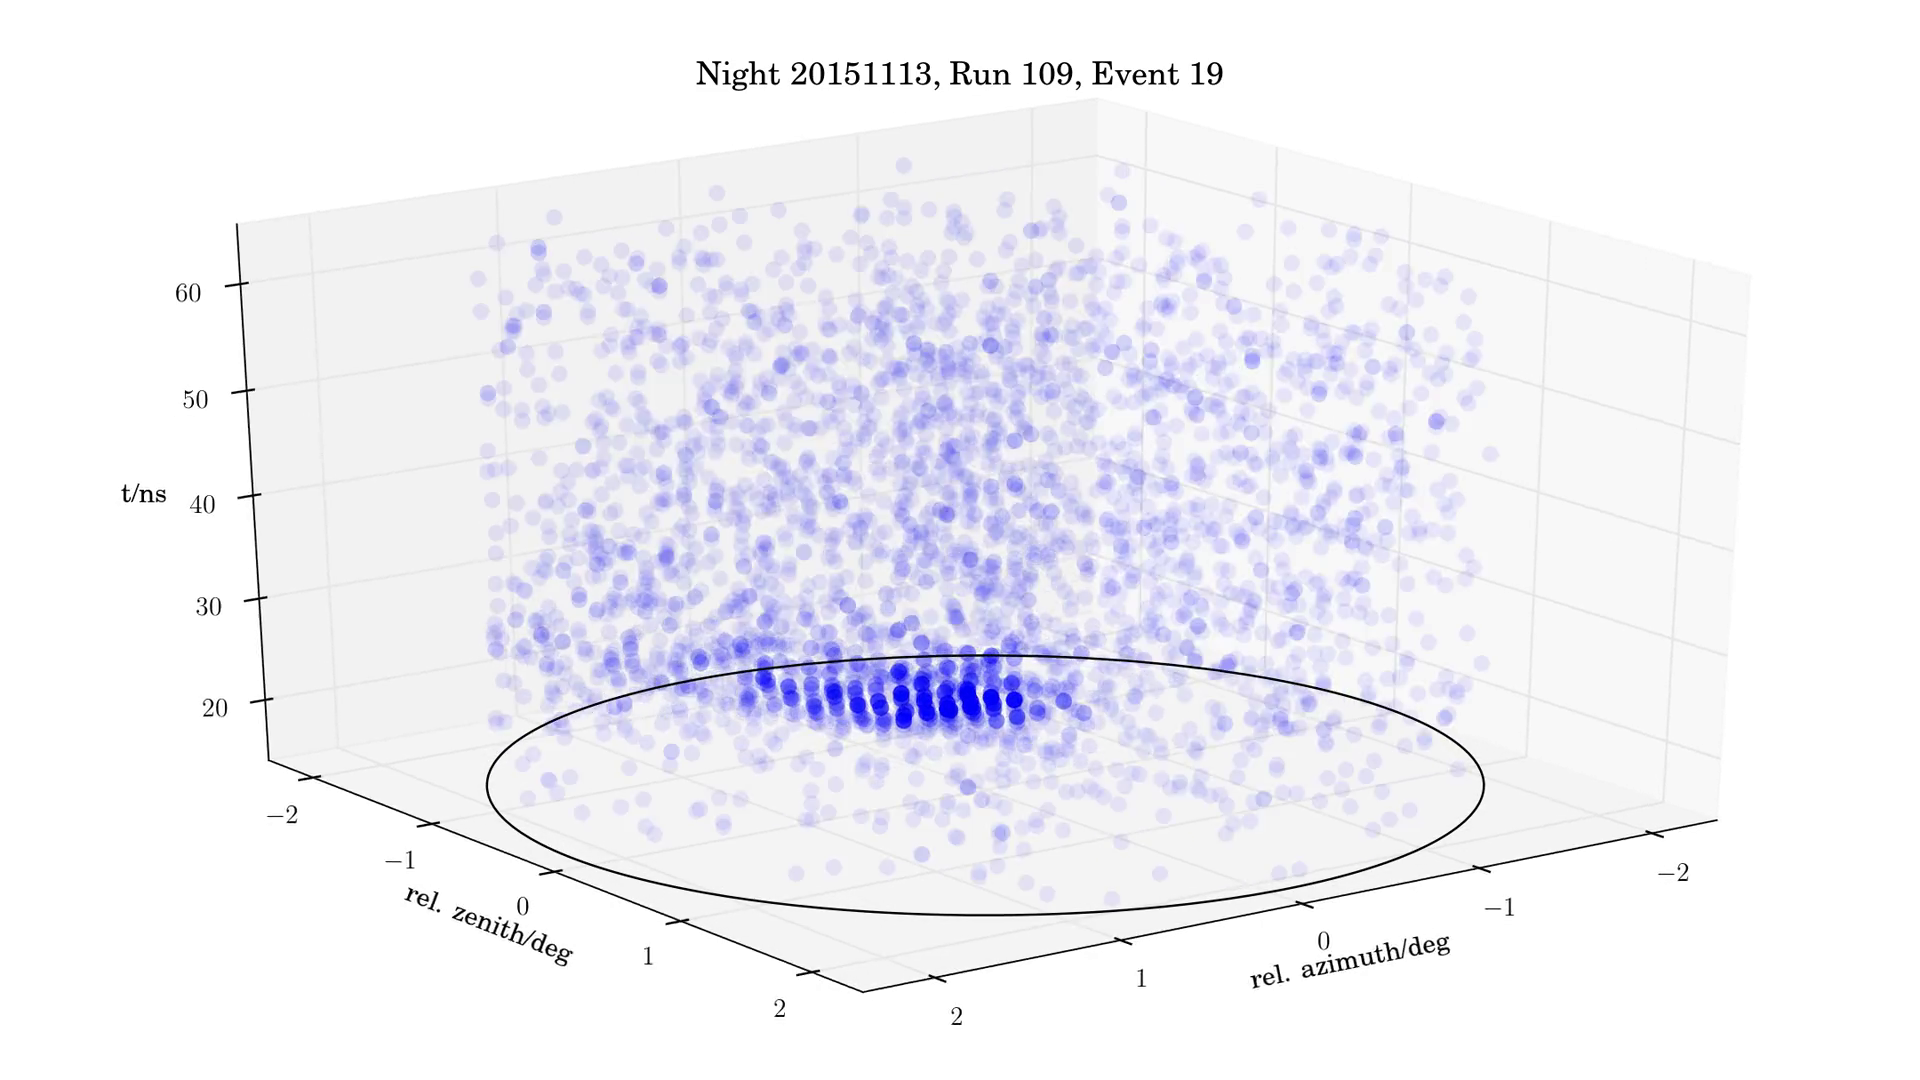
\includegraphics[width=1.2\textwidth]{fig/event2.png}
            \onslide<2>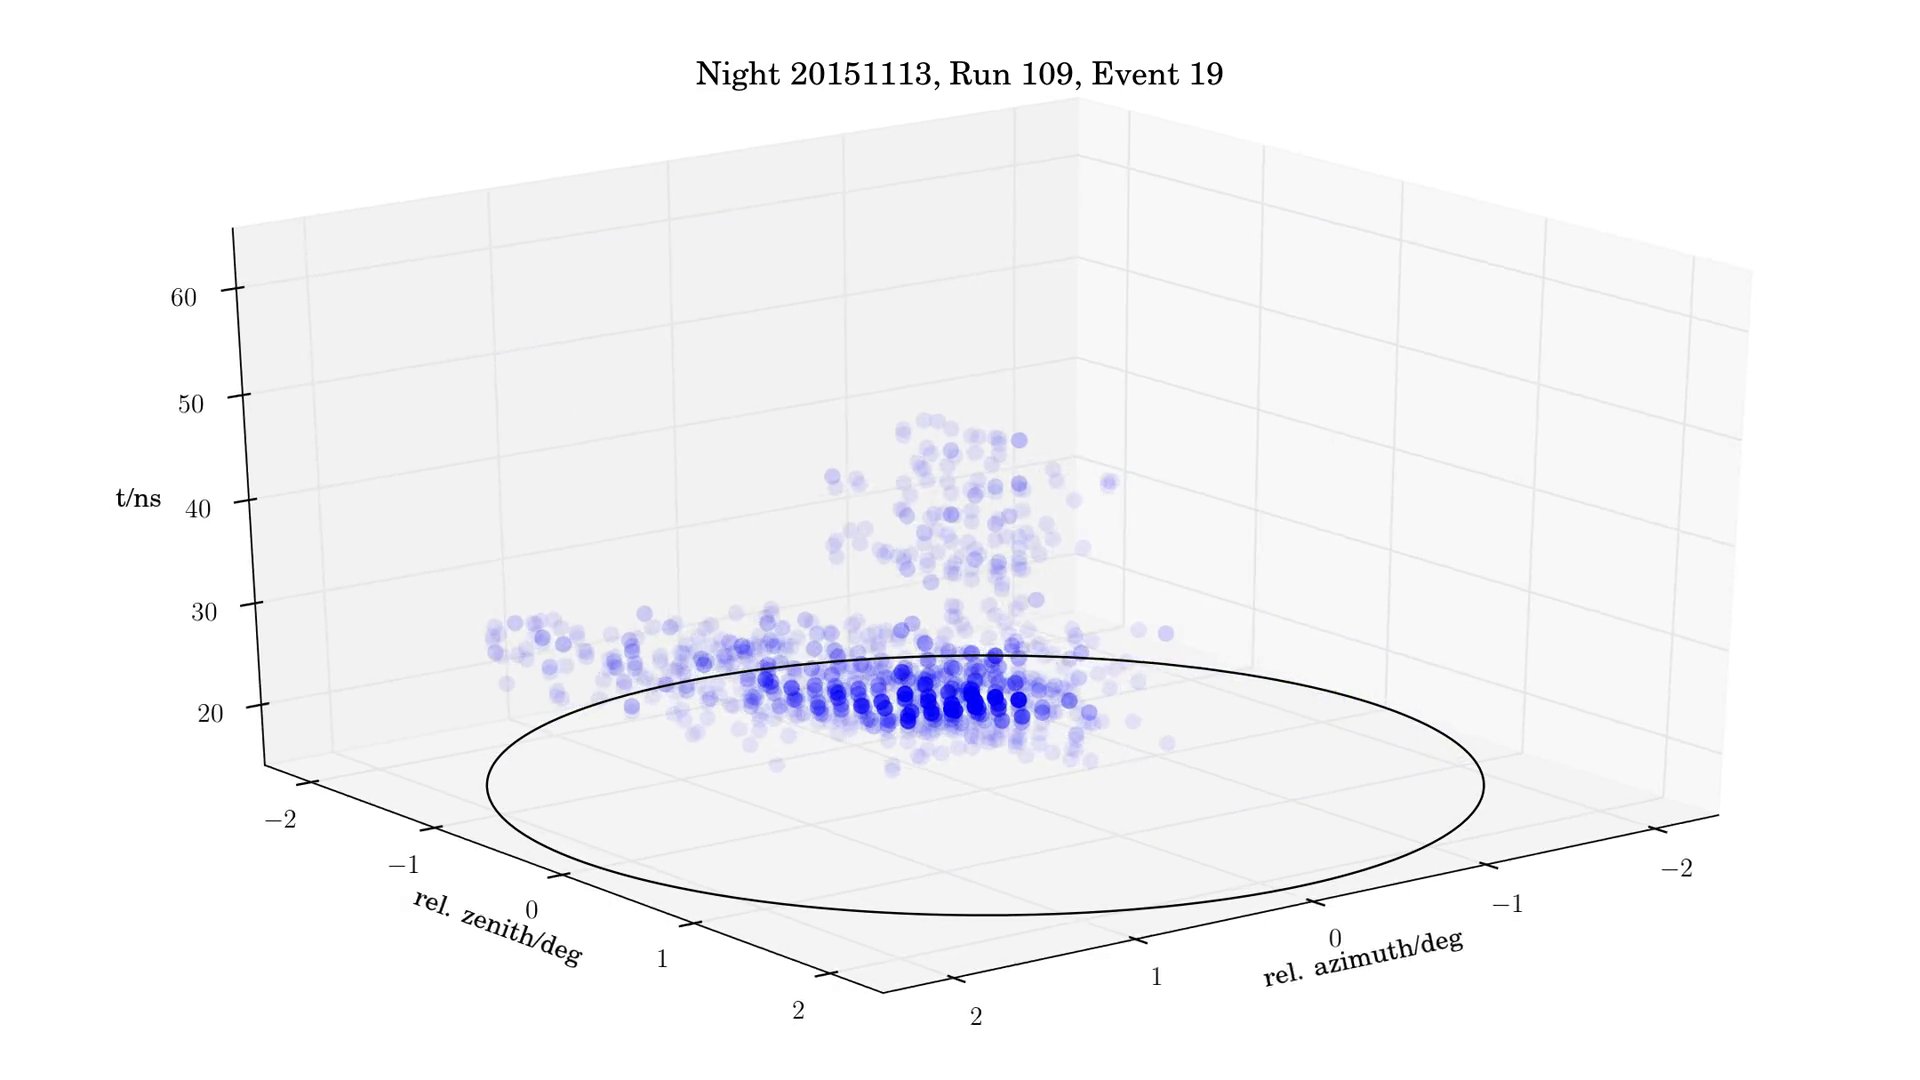
\includegraphics[width=1.2\textwidth]{fig/event1.png}
        \end{overprint}
    \end{column}
    \begin{column}{0.475\textwidth}
        \begin{itemize}
            \vspace*{\fill}
            \item smaller file size: possible to compress all FACT data to fit on one 10TB drive
            \item simplify \textit{exchange} and \textit{analysis}, gain timing knowledge
            \item DBSCAN: cluster based image cleaning
            \item exptected improvement for cleaning
            % \item do physics analysis on an SiPM based IACT
        \end{itemize}
    \end{column}
\end{columns}
\end{frame}



\section{Data Set: FACT open data crab sample}

\begin{frame}[t]{The Data set: FACT open data crab sample}
\begin{columns}[onlytextwidth]
    \begin{column}{0.475\textwidth}
        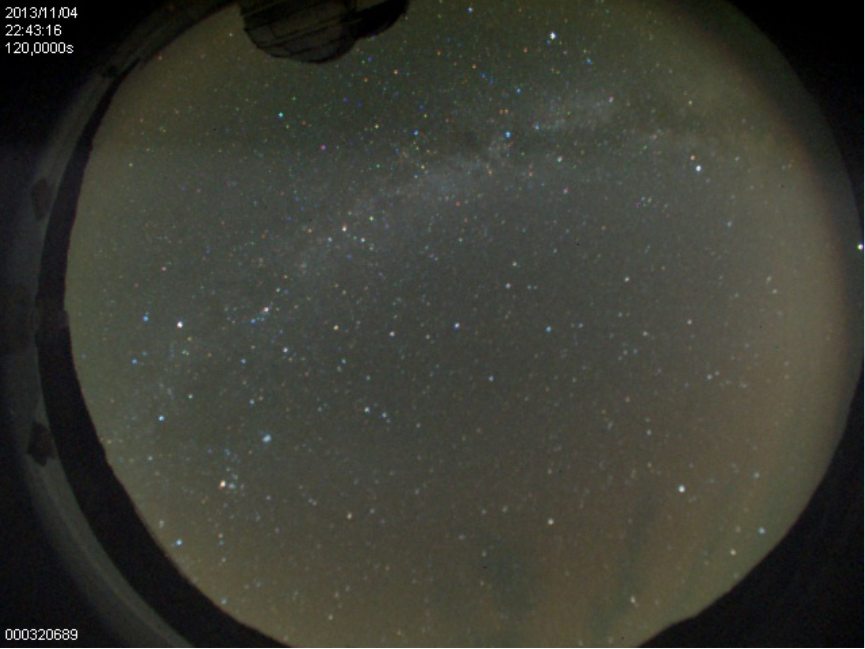
\includegraphics[width=\textwidth]{fig/cond.png}
    \end{column}
    \begin{column}{0.475\textwidth}
    \vspace*{\fill}
        \begin{itemize}
            \item \url{https://fact-project.org/data}
            \item Crab Nebula observations from November 2013
            \item including gamma-ray and proton simulations
            \item $17.7$ hours of observations
        \end{itemize}
    \end{column}
\end{columns}
\end{frame}

\section{Analysis}

\begin{frame}[t]{Analysis}
\begin{description}[Crab Nebula]
    \item[aim] proof of concept: generate preliminary physics results
    \item[Crab Nebula] well measured source of cosmic gamma rays $\rightarrow$ standard candle analysis
\end{description}
\vspace{\fill}
\begin{columns}[onlytextwidth]
    \begin{column}{0.475\textwidth}
        \textbf{{\color{tugreen} \underline{Standard Analysis chain}}}
        \begin{description}[parametrization]
            \item[calibration] identifying large pulses
            \item[image cleaning]
            \item[parametrization] Hillas
            \item[separation]
            \item[reconstruction]
        \end{description}
    \end{column}
    \begin{column}{0.475\textwidth}
        \textbf{{\color{tugreen} \underline{Photon Stream Analysis chain}}}
            \begin{description}[parametrization]
                \item[calibration] extracting single photons
                \item[image cleaning] DBSCAN
                \item[parametrization] Hillas
                \item[separation]
                \item[reconstruction]
            \end{description}
    \end{column}
\end{columns}
\end{frame}

\begin{frame}[t]{Parameterization}
\begin{columns}[onlytextwidth]
    \begin{column}{0.475\textwidth}
        \vspace{20px}
        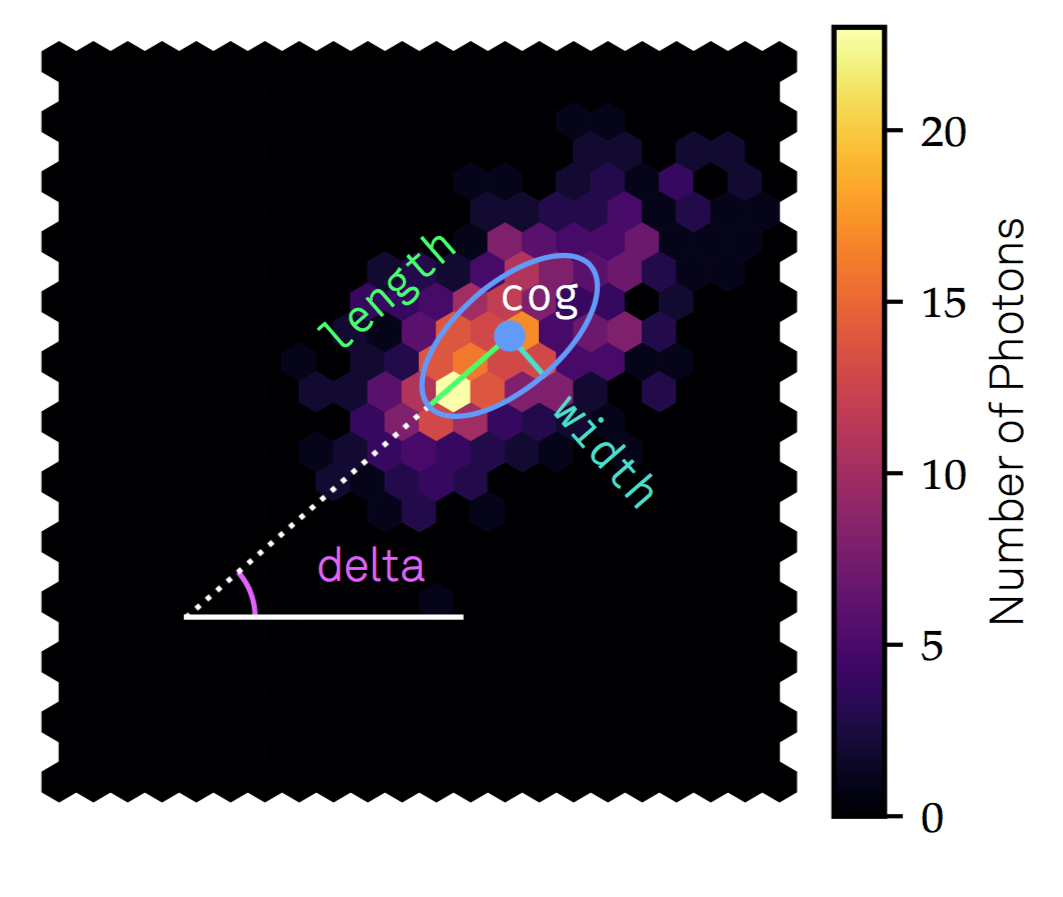
\includegraphics[width=0.98\textwidth]{fig/hillas.png}
    \end{column}
    \begin{column}{0.475\textwidth}
    Hillas parameters (projected back to 2D): \\
        \begin{itemize}
            \setlength\itemsep{1em}
            \item \textbf{{\color{tugreen} size}}: number of photons in cluster
            \item \textbf{{\color{tugreen} length}}: std. dev. along long half-axis
            \item \textbf{{\color{tugreen} width}}: std. dev. along short half-axis
            \item \textbf{{\color{tugreen} delta}}: angle between length and disp
            \item \textbf{{\color{tugreen} skewness/ kurtosis}}: higher order statistical moments along half-axes in cluster system
        \end{itemize}
    \end{column}
\end{columns}
\end{frame}

\begin{frame}[t]{Parameterization}
    \begin{columns}[onlytextwidth]
        \begin{column}{0.475\textwidth}
            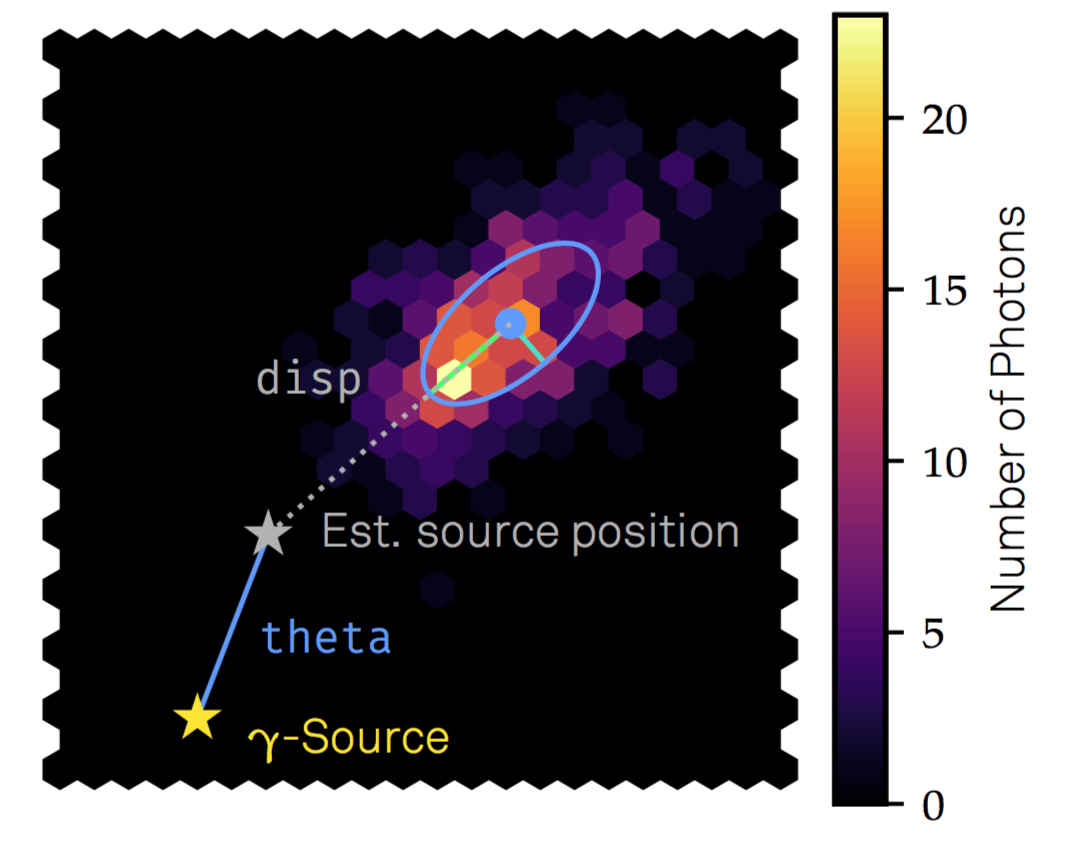
\includegraphics[width=\textwidth]{fig/disp.png}
        \end{column}
        \begin{column}{0.475\textwidth}
            Source position reconstruction via disp-method:
            \begin{itemize}
                \item \textbf{{\color{tugreen} |disp|}}: distance from centre of gravity to target
                \item \textbf{{\color{tugreen} sgn(disp)}}: Head/Tail-Disambiguation
                \item \textbf{{\color{tugreen} theta}}: distance between reconstructed and true origin
            \end{itemize}
        \end{column}
    \end{columns}
\end{frame}

\begin{frame}[t]{Tools}
Machine learning with FACT classifier-tools, using 5-fold cross validation  \url{https://github.com/fact-project/classifier-tools} \\
\textbf{{\color{tugreen} Energy estimation}}:
\begin{itemize}
    \item random forest regressor (30 estimators)
\end{itemize}
\textbf{{\color{tugreen} Gamma-hadron-separation}}:
\begin{itemize}
    \item random forest classifier (50 estimators)
\end{itemize}
\textbf{{\color{tugreen} Origin reconstruction}}:
\begin{itemize}
    \item two step task: regression of |disp| and classification of sgn(disp)
    \item random forest regressor and classifier
\end{itemize}

\begin{block}{Open Crab Sample Analysis}
    \url{https://github.com/fact-project/open_crab_sample_analysis}
\end{block}
\end{frame}

\section{Results}
\begin{frame}[t]{Energy estimation}
\begin{columns}[onlytextwidth]
    \begin{column}{0.475\textwidth}
        \vspace{-25px}
        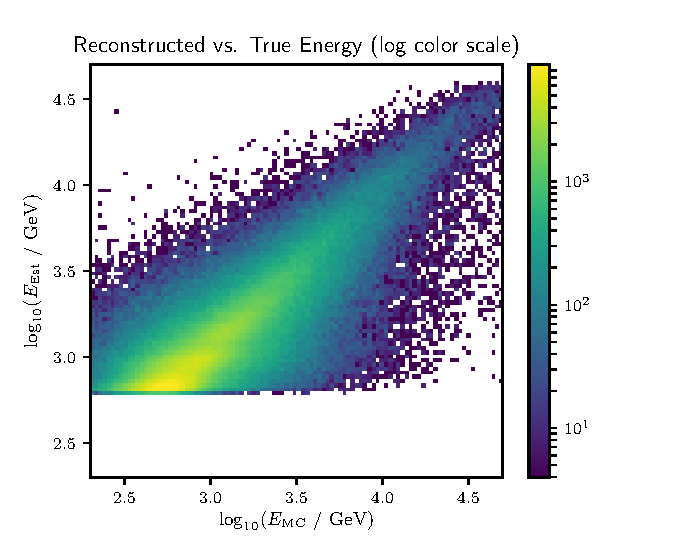
\includegraphics[width=1.15\textwidth,page=1]{fig/energy_performance.pdf}
    \end{column}
    \begin{column}{0.475\textwidth}
        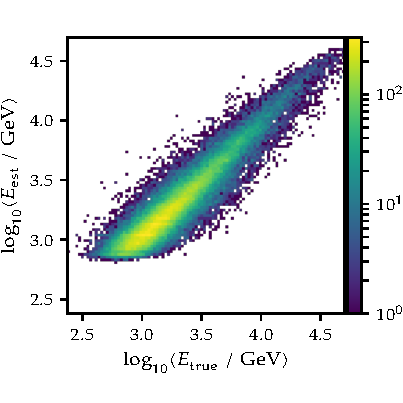
\includegraphics[width=\textwidth]{fig/energy_migration.pdf}
    \end{column}
\end{columns}
\end{frame}

\begin{frame}[t]{Separation}
\begin{columns}[onlytextwidth]
    \begin{column}{0.475\textwidth}
        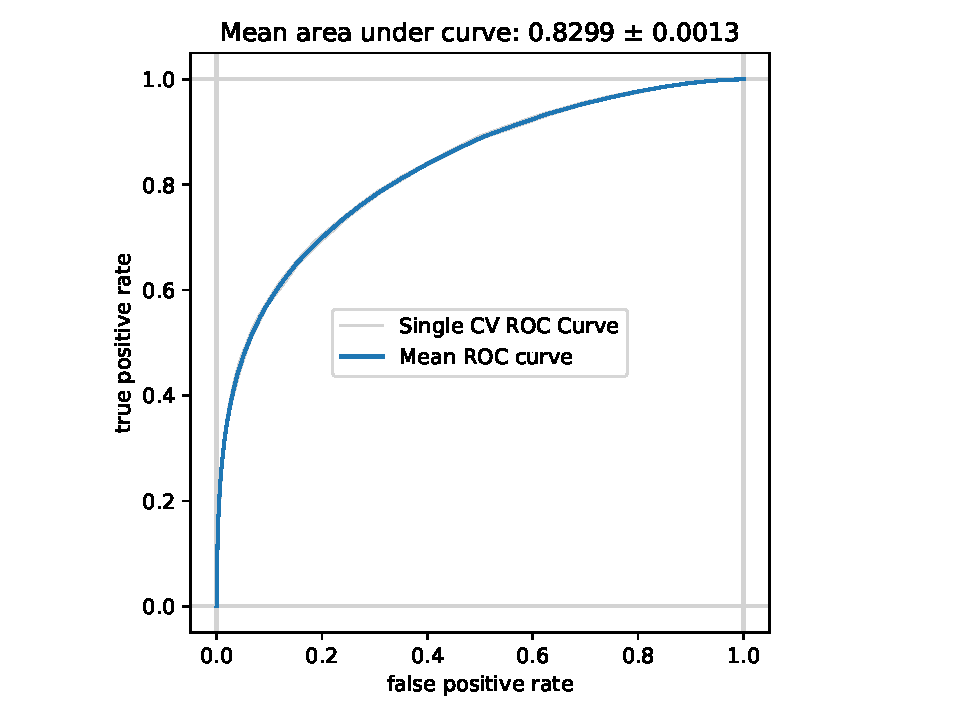
\includegraphics[width=\textwidth,page=1]{fig/separation_performance.pdf}
    \end{column}
    \begin{column}{0.475\textwidth}
        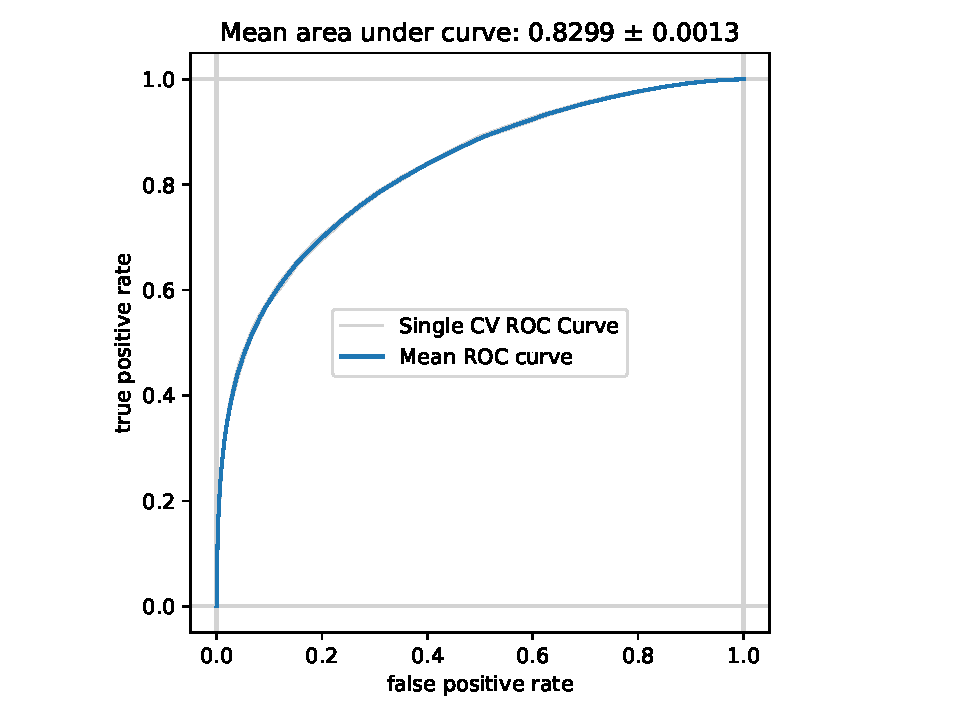
\includegraphics[width=\textwidth,page=1]{fig/separation_performance.pdf}
    \end{column}
\end{columns}
\end{frame}

\begin{frame}[t]{Origin reconstruction}
\begin{columns}[onlytextwidth]
\begin{column}{0.475\textwidth}
    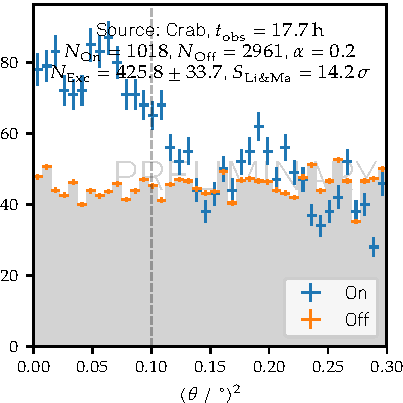
\includegraphics[width=\textwidth]{fig/theta2_plot.pdf}
\end{column}
\hfill%
\begin{column}{0.475\textwidth}
    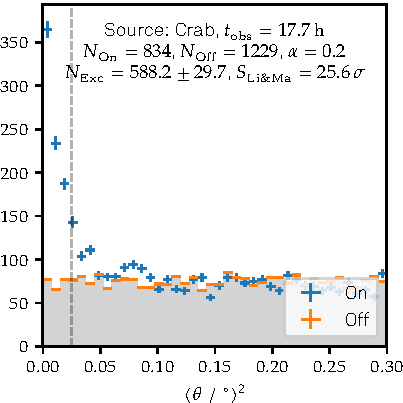
\includegraphics[width=\textwidth]{fig/theta2.pdf}
\end{column}
% \begin{itemize}
%     \item mean accuracy for sgn(disp): $\SI{83}{\percent}$
%     \item mean $\text{R}^2$ score for disp: $0.624\,\pm\,0.003$
% \end{itemize}
\end{columns}
\end{frame}


\section{Summary}



\begin{frame}[t]{Summary}
    \begin{columns}[onlytextwidth]
        \begin{column}{0.3\textwidth}
            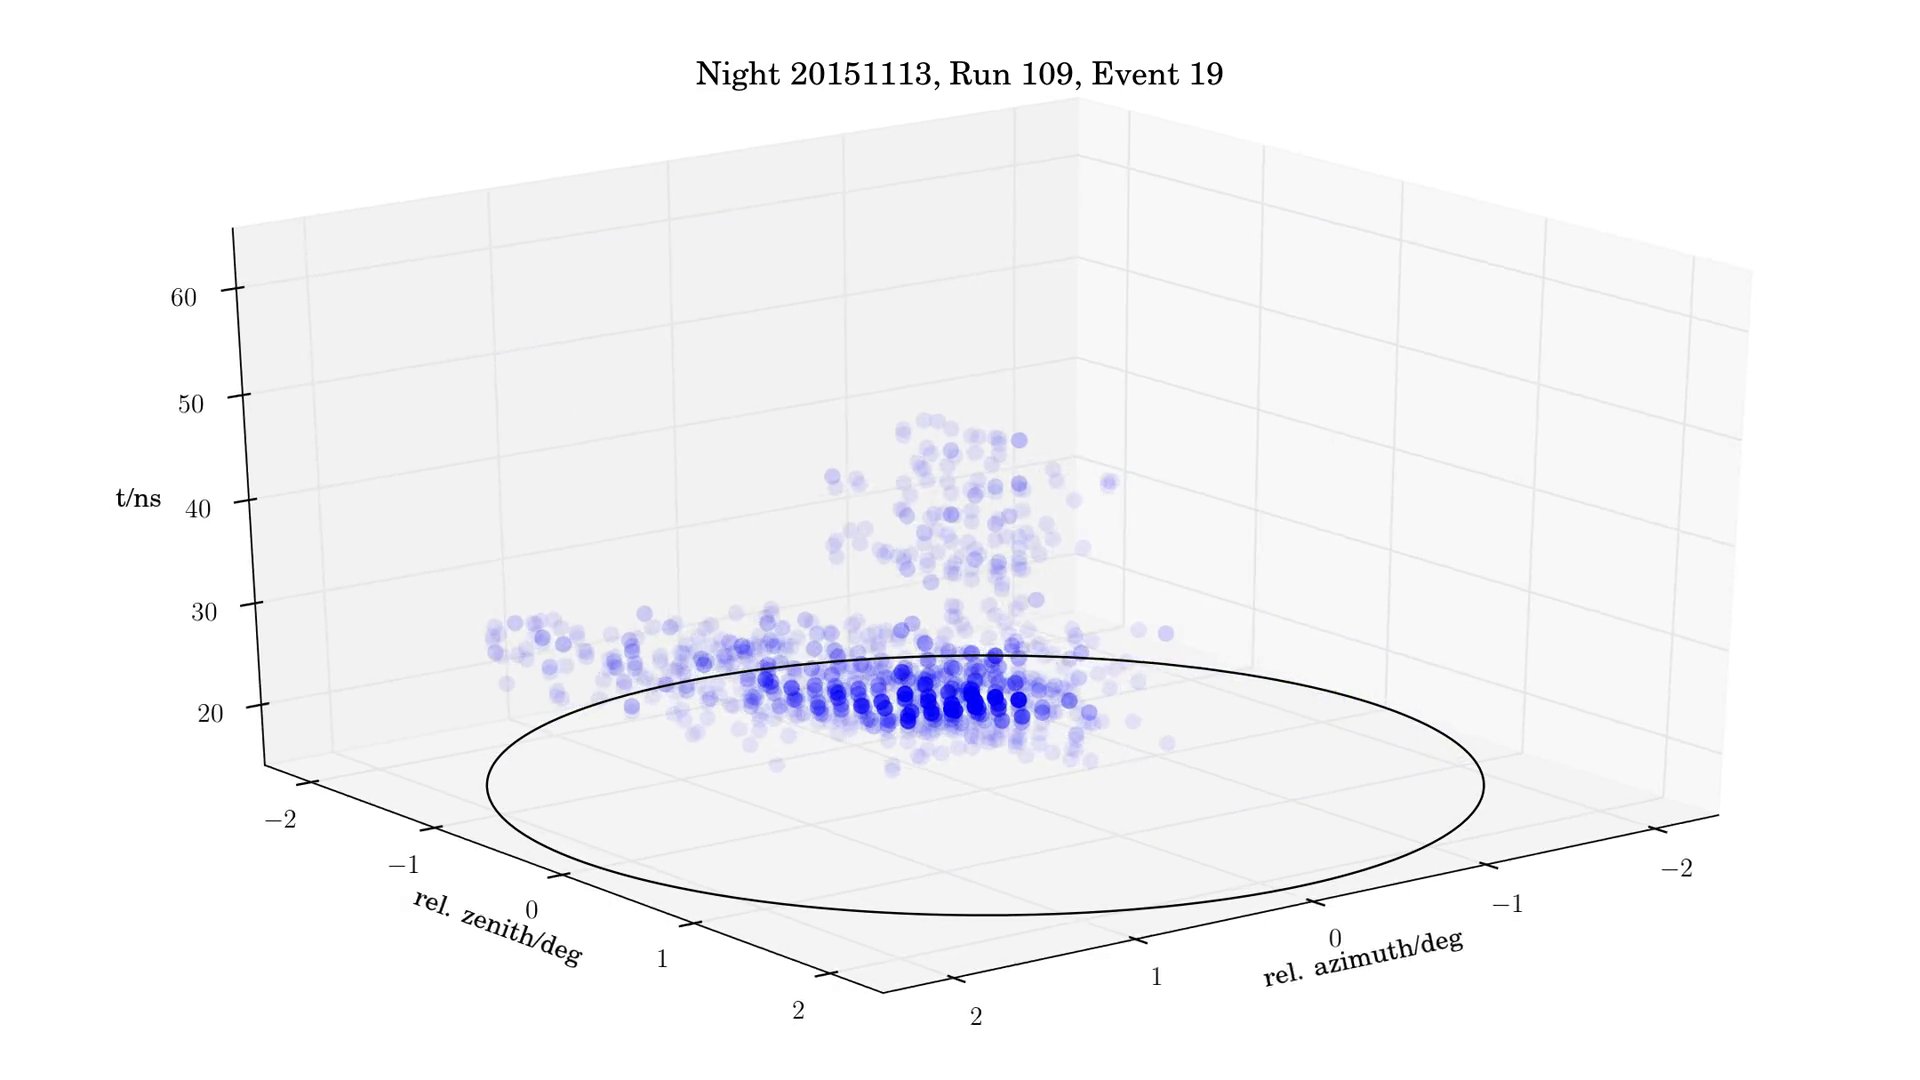
\includegraphics[width=1.2\textwidth]{fig/event1.png}
        \end{column}
        \begin{column}{0.3\textwidth}
            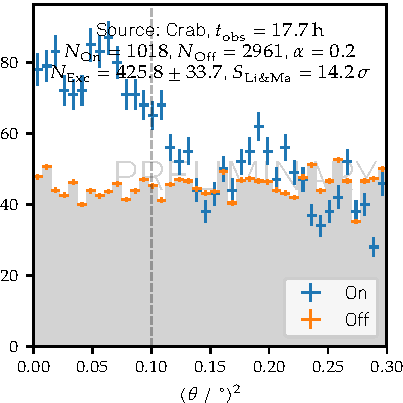
\includegraphics[width=\textwidth]{fig/theta2_plot.pdf}
        \end{column}
        \begin{column}{0.3\textwidth}
            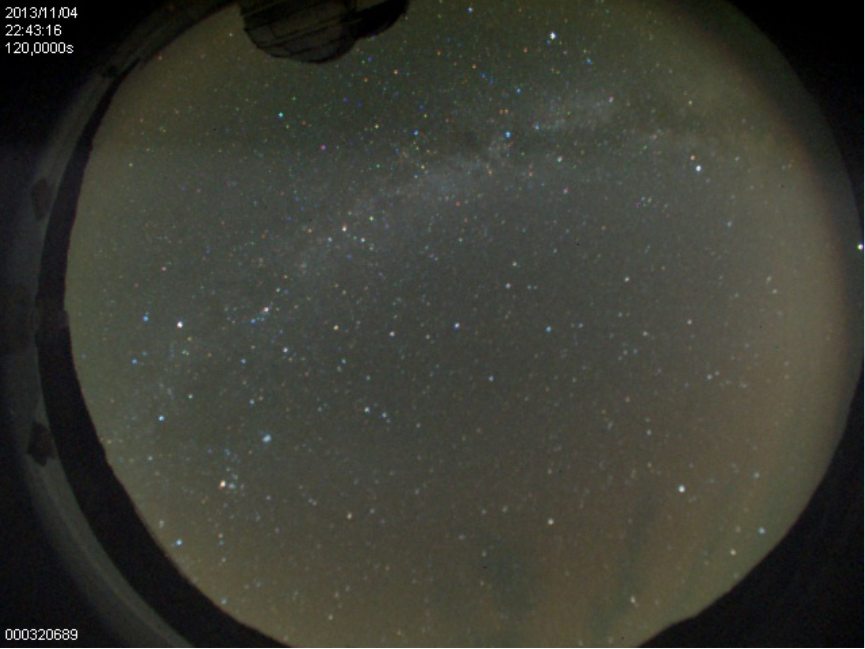
\includegraphics[width=\textwidth]{fig/cond.png}
        \end{column}
    \end{columns}
% \vfill%
\textbf{{\color{tugreen} Outlook}} \\
This is just the beginning!
\begin{itemize}
    \item improve feature selection $\rightarrow$ feature engineering
        \begin{itemize}
            \item[$-$] implement more "standard" features
            \item[$-$] timing information (3-dimensional point-cloud)
        \end{itemize}
    \item improve cuts on data, hyper-parameters of classifier-tools and clustering
\end{itemize}
\end{frame}
% Works well already! \\
% \begin{table}
%   \centering
%   \begin{tabular}{c
%                   c
%                   S[table-format=1.2]
%                   S[table-format=1.4(2)]
%                   S[table-format=1.4(2)]}
%     \toprule
%     {} & {significance crab} & {separation AUC ROC} & {sign accuracy} & {disp $\text{R}^2$} \\
%     \midrule
%     This analysis & $14.2\,\sigma$ & 0.87 & 0.83  & 0.624(3)  \\
%     Std analysis & $24.2\,\sigma$ & 0.89 & 0.75        & 0.6(2)  \\
%     \bottomrule
%   \end{tabular}
% \end{table}
% \vspace{10px}
% \textbf{{\color{tugreen} Comparison with FACT standard analysis}}
% \begin{itemize}
%     \item significance on crab sample detection: $24.2\,\sigma$ as compared to $X\,\sigma$
%     \item separation AUC ROC: $0.89$ as compared to $0.83$ (this analysis)
%     \item disp method:
% \end{itemize}



% %-------------------------------------------------------------------------------
% \section{Back up}
% %-------------------------------------------------------------------------------
% \appendix
%
% \begin{frame}[t]{}
%   \centering
%   \textcolor{tugreen}{\Huge{Back Up}}
% \end{frame}

\end{document}
